%% It is just an empty TeX file.
%% Write your code here.

\documentclass[12pt]{article}
\usepackage[margin=1in]{geometry}
\usepackage{amsfonts, amsmath, amssymb}
\usepackage[none]{hyphenat}
\usepackage{fancyhdr}
\usepackage{graphicx}
\usepackage{cite}
\usepackage{caption}
\usepackage{subcaption}
\usepackage{lastpage}
\usepackage{setspace}

\DeclareMathOperator*{\argminA}{arg\,min} % Jan Hlavacek
\DeclareMathOperator*{\argminB}{argmin}   % Jan Hlavacek


\begin{document}

\thispagestyle{empty}
\vspace*{1\baselineskip}
\centerline{\bf{WASHINGTON UNIVERSITY IN ST.LOUIS}}
\vspace*{1\baselineskip}
\centerline{Department of Mathematics}
\vspace*{8\baselineskip}
\centerline{Statistical Models to Predict Popularity of News Articles on Social Networks}
\vspace*{2\baselineskip}
\centerline{by}
\vspace*{1\baselineskip}
\centerline{\bf{Ziyi Liu}}
\vspace*{12\baselineskip}
\centerline{A thesis presented to the}
\centerline{Graduate School of Arts and Sciences} 
\centerline{of Washington University in}
\centerline{partial fulfillment of the}
\centerline{requirements for the}
\centerline{degree of Master of Arts}
\vspace*{4\baselineskip}
\centerline{May 2017}
\vspace*{1\baselineskip}
\centerline{St. Louis, Missouri}
\clearpage

\doublespacing

\pagenumbering{roman}
\setcounter{page}{2}
\tableofcontents
\newpage

\listoffigures
\newpage

\listoftables
\clearpage

\addcontentsline{toc}{section}{Acknowledgements}
\vspace*{1\baselineskip}
\centerline{\bf{Acknowledgements}}
\vspace*{4\baselineskip}
I would like to sincerely thank Prof. Kuffner for his patience and kindness. She always provides me lots of valuable ideas and suggestions. It would be impossible for me to accomplish this thesis without his help and guidance.
\vspace*{1\baselineskip}

In addition, I would like to express my gratitude to all the faculty, staff, and friends in our Math Department. They are so kind to me and make me feel warm as a member of the Math Department.
\vspace*{1\baselineskip}

Last but not least, I would like to thank my parents for their love and support. I gained and learned so much from you.

\vspace*{4\baselineskip}
\centerline{Ziyi Liu}
\centerline{Washington University in St. Louis, 2017}
\centerline{May 2017}

\newpage


\addcontentsline{toc}{section}{Abstract}
\centerline{\bf{Abstract of the Thesis}}
\vspace*{1\baselineskip}
\centerline{\bf{Statistical Models to Predict Popularity of News Articles on Social Networks}}
\vspace*{1\baselineskip}
\centerline{by}
\vspace*{1\baselineskip}
\centerline{\bf{Ziyi Liu}}
\vspace*{1\baselineskip}
\centerline{\bf{Master of Arts in Statistics}}
\vspace*{1\baselineskip}
\centerline{Washington University in St. Louis, 2017}
\vspace*{1\baselineskip}
\centerline{Professor Todd Kuffner, Chair}
\vspace*{2\baselineskip}
Social networks have changed the way that we obtain information. Content creators and, specifically news article authors, have in interest in predicting the popularity of content, in terms of the number of shares, likes, and comments across various social media platforms. In this thesis, I employ several statistical learning methods for prediction. Both regression-based and classification-based methods are compared according to their predictive ability, using a database from the UCI Machine Learning Repository.\\
\vspace*{1\baselineskip}
\vspace*{1\baselineskip}

{\bf{Key words:}} Statistical Models, News Articles, Social Networks
\newpage
\setcounter{page}{1}
\pagenumbering{arabic}
\section{Introduction}
As we know, Most people get information and knowledge from news and articles. In this era, people are also used to using through the internet to do everything. So it’s no doubt that online news and articles are playing a very important role in our daily life. We can get any news we want through internet quickly. Also, it’s much easier to figure out which online news or articles we like through many internet outlets, such as shares, likes and comments. 

As we can imagine, popular news can make the authors become famous, also it can help the social media company attract more people. So they can make more profits. So if an author can know what can make news or articles become popular, or one company can predict whether news or articles will be popular before them are published, they will definitely try their best to get the information. 

So this project aims to find a method to predict the popularity of an online article before it is published by using several statistic characteristics summarized from it. We use a dataset from UCI Machine Learning Repository. In this dataset, it uses the number of shares for an online article to measure how popular it is. It contains 39644 observations with 60 variables, including 2 variables that are not used in other studies involving this dataset. We use one of these additional variables to build our predictive model. 

The input of the algorithm is several features of Mashable articles: Words (e.g. number of words in the title), Links (e.g. number of Mashable article links), Digital Media (e.g. number of images), Time (e.g. day of the week), Keywords (e.g. number of keywords) and Natural Language Processing (e.g. closeness to top 5 LDA topics). \cite{fernandes2015proactive}

We will predict the popularity in two perspectives. Firstly, we can use regression models(e.g. regression, GAM, Lasso) to predict the number of shares. Secondly, we categorize articles into 3 levels (unpopular, normal, popular) and then use a classification algorithm(e.g. SVM, Random Forest, KNN) to predict the article's popularity level.  

\newpage
\section{Method}
\subsection{K-fold cross-validation} 
Before we talk about any statistical models, we first introduce some methods for model selecting. K-fold cross-validation is a method for estimating prediction error. \\
If we had enough data, we could set a dataset and use it to evaluate our prediction model. But we always can't get as many data as we want. To deal this problem, K-fold cross-validation uses part of the data we have to build the model, and another part to test it. We split the data randomly into K parts which are almost the same size. For example, we let K = 10. For the kth part, we train the model by the rest K-1 parts of data, and let $\hat{f}^{-k}(x)$ be the fitted function, where $x_{-k}$ is the dataset excluding the kth part. Then we use this model to predict the kth part of data and get the mean squared prediction error (MSPE) for kth part:$$MSPE_k = \frac{1}{n_k} \sum_{i=1}^{n_k} (y_j - \hat{f}^{-k}(x_j))^2,$$ where $n_k$ is the number of observations in the kth part of data, $y_j$ is the response of jth observation in the kth part of data, $x_j$ is the predictors of jth observation in the kth part of data. Then we get K MSPEs, so we can get the K-fold cross-validation estimate: $$CV_{K} = \frac{1}{K} \sum_{k=1}^{K} MSPE_k.$$ \\
Given a set of models $f(x, \alpha)$ indexed by a tuning parameter $\alpha$, we can use this method to find the best value for $\alpha$. \cite[p.241-245]{friedman2001elements}

\subsection{Confusion matrix}
Confusion matrix is a matrix which shows predicted and actual classifications. The size of a confusion matrix is N $\times$ N, where N is the number of different classes. \cite{kohavi1998glossary, altman1994diagnostic} We can see how many observations are correctly or incorrectly classified. The elements in the diagonal of the confusion matrix indicate correct predictions, while the off-diagonal elements are incorrect predictions. So we can get the accuracy which is the percentage of correct predictions from all predictions. One way to getting the better model is choosing the one which has higher accuracy. \cite{james2013introduction}

\subsection{Linear models}  
Linear models are still used in statistical learning as a first approximation, before trying more complicated method. So firstly, we try to use ordinary least squares (OLS) estimates the result. If we have an input vector $X^T=(X_1,X_2,...,X_p)$, and want to predict a output Y. The linear regression model has the form $$Y=\beta_0+\sum_{j=1}^{p} X_j\beta_j + \epsilon$$
The linear model has several assumptions. The regression function E(Y$\mid$X) is linear or it's reasonable to approximate it into linear model. In this formula, $\beta_j$s are unknown parameters, and variables $X_j$ can be in different sources. 
Also, we always assume that E(Y$\mid$X)=f(X) is a linear function of X and the error follows $\epsilon \sim \mathcal N(0, \sigma^2I)$ and $\epsilon$ uncorrelated with X and X is full rank which implies that $X^TX$ is nonsingular and positive definite. \cite[p.44-49]{friedman2001elements} 

\subsection{Least Absolute Selection and Shrinkage Operator(lasso)}  
Lasso is another way for least squares estimation in linear models. As we know, OLS estimation can have low bias, but it also give a large variance. If we shrink several variable coefficients to 0, we can trade a little bit bias in order to get a smaller variance, so we may get a better prediction accuracy. Also, when we set several variable coefficients to 0, we can use a smaller subset to interpret results to show the strongest effects. For this method, we assume that $x_{ij}$ are standardized and $\bar y = 0$ \\
It solves the problem $$\min_{\beta} \sum_{i=1}^{n} (y_i-\sum_{j=1}^{p} x_{ij}\beta_{ij})^2 \text{, subject to } \sum_{j=1}^{p} \lvert \beta_j \rvert \leq t.$$
Where t $\geq$ 0 is a parameter given by users. It controls the amount of shrinkage that is applied to the estimates. For the full least squares estimates $\hat{\beta}^0_j$, we can get $t_0=\sum_{j=1}^{p} \lvert \hat{\beta}^0_j \rvert$. $\forall t \leq t_0$, if we think about orthonormal design case, which we let X be the matrix with n$\times$p and $X^TX = I$, the solution for the previous equation is $$\hat{\beta_j}=\text{sign}(\hat{\beta}^0_j)(\lvert \hat{\beta}^0_j \rvert - \gamma)^+$$ where $\gamma$ is determined by the condition $\sum_{j=1}^{p} \lvert \hat{\beta_j} \rvert = t$. We can easily see that some $\hat{\beta_j}$ will go to 0. \\
In order to get the lasso solution, we let $g(\beta)=\sum_{i=1}^{n} (y_i - \sum_{j} \beta_jx_{ij})^2$, and let $\delta_i$, i=1,2,...,$2^p$ be the p-tuples of the form $(\pm1,\pm1,...,\pm1)$. Then we know that $\sum_j \lvert \beta_j \rvert \leq t$ is equivalent to $\delta_i^T \beta \leq t$ for all i. For a given $\beta$, let $E=\{i:\delta_i^T \beta = t\}$ and $S=\{i:\delta_i^T \beta < t\}$. The set $E$ called equality set, which exactly meets the constraints, while $S$ is the slack set, which does not hold the equality. Denote by $G_E$ the matrix whose rows are $\delta_i$ for $i \in E$. Let $\vec{1}$ be a vector of 1s of length equal to the number of rows of $G_E$. \\
Then the algorithm starts with $E=\{i_0\}$ where $\delta_{i_0}=\text{sign}(\hat \beta^0)$. Then we find $\hat \beta$ to minimize $g(\beta)$ subject to $G_E \beta \leq t \vec{1}$. If $\sum \lvert \beta_j \rvert \leq t$, we finished; if not, add i to the set $E$ where $\delta_i=\text{sign}(\hat \beta)$. Then the previous step again, until $\sum \lvert \beta_j \rvert \leq t$.
 \cite{tibshirani1996regression}  

\subsection{Generalized Additive Models(GAM)} 
Linear models are good, but as the effects are often not linear in the real world, linear models often fail. We can use some more flexible statistical methods that can show nonlinear effects. We call these methods "generalized additive models". In general, if we have an input vector $X^T=(X_1,X_2,...,X_p)$ and want to predict a output Y, we can use a link function $g$ to relate the condition mean $\mu(X)$ of Y to an additive function: $$g[\mu(X)] = \alpha + f_1(X_1) + ... + f_p(X_p).$$ In this thesis, we use $g(\mu) = \mu$, the identity link, for the response data. So the additive model has the form $$Y=\alpha+\sum_{j=1}^{p} f_j(X_j)+\epsilon,$$
where the mean of error term $\epsilon$ is 0. As each $f_j$ is an unspecified smooth nonparametric function. The approach is using an algorithm for simultaneously estimating all functions instead of expanding each function then fitted by simple least squares. Given observation $x_i$, $y_i$, the criterion is : $$\text{PRSS}(\alpha,f_1,...,f_p) = \sum_{i=1}^{N} (y_i-\alpha-\sum_{j=1}^{p}f_j(x_{ij}))^2+\sum_{j=1}^{p} \lambda_jf_j(x_{ij}),$$ where the $\lambda_j \leq 0$ are tuning parameters. It can be shown that the minimizer of the previous equation is an additive cubic spline model. \cite[p.295-299]{friedman2001elements} 

\subsection{Support Vector Machines(SVM)}  
Besides the regression models, we also utilized classification algorithms for prediction. Support Vector Machines are a technique for constructing an optimal separating hyperplane between two classes. For two classes data, for example if this data can be perfectly separated, we can find infinitely many possible linear boundaries to separate the data. These linear boundaries are separating hyperplanes. \cite[p.129-130]{friedman2001elements} And we can find an optimal separating hyperplane, which can make the margin which is defined as $1/\lVert \beta \rVert$ maximize, where $\beta$ is the vector for each variable coefficients. \\
So we can define SVM model with the Lagrange dual objective function:$$\text{max }L(\alpha)=\sum_{i=1}^{n} \alpha_i - \frac{1}{2}\sum_{i=1}^{n}\sum_{i'=1}^{n}\alpha_i \alpha_{i'} y_i y_{i'} K(x_i,x_{i'}).$$
    Where we use $\alpha_i$ to represent $\beta$. s.t. $$\beta = \sum^{n}_{i=1} \alpha_i y_i x_i$$
$$0=\sum_{i=1}^{n} \alpha_iy_i $$
$$0 \leq \alpha_i \leq C $$
And the $K(x_i,x_{i'})$ is the kernel function. For this dateset, I try to use linear kernel and radial kernel. As linear is the simplest one and radial kernel is the most popular choice for Gaussian. 
    \begin{align}
        &\text{linear kernel}  &K(x_i,x_{i'})=<x_i,x_{i'}> \nonumber \\
        &\text{radial kernel}  &K(x_i,x_{i'})=exp(-\gamma \lVert x_i-x_{i'} \rVert^2) \nonumber
    \end{align}
For a multiclass classification, if we have K classes total, we can put each two class together to train a decision boundary. So we can build K(K-1)/2 decision boundaries to decide one point should be put in which class. This method is called one vs one SVM model. \cite[p.417-431]{friedman2001elements}

\subsection{Random Forest} 
Before we talking about Random Forest, we need to decribe tree-based methods first.\\ 
Generally speaking, tree-based methods for predicting $y$ from a feature vector $x\in \mathbb{R}^p$ split the feature space into a set of rectangles, and then fit a simple model in each one. \cite[p.305-310]{friedman2001elements} \\
Then we introduce the bagging method. The essential idea for bagging is that if we have B separate uncorrelated training sets, we could form B separate models, and use the average or mode as the final model. So in tree-base model, we take B datasets whose observations are all getting from the training set randomly and with replacement and the size is same as the original training dataset. So we can use B different datasets to build B different trees. Then we use the most frequent result to give the predictions. \cite[p282-283]{friedman2001elements} \\
Random Forest is imporved from bagging. For growing the tree from the datasets we generated, we select m variables at random from the p variables, instead of using all p variables to pick the best variables/split-point. As all datasets are just identically distributed, but not independent, they will have a positive pairwise correlation $\rho$, the variance of the average is $$\rho\sigma^2+\frac{1-\rho}{B}\sigma^2.$$ As B increases, the variance goes to first term. The idea in random forest is to reduce the variance compared with bagging, by reducing the correlation between the trees, without increasing the variance too much. \cite[p.606-607]{friedman2001elements}

\subsection{K-Nearest Neighbors(KNN)} 
This idea can be used both in regression and classification. The main idea is we try to estimate the result of $x_0$ using the k training points $x_{(r)}, r=1,...,k$ which are nearest to the $x_0$. For this dataset, we use Euclidean distance $$d_{(i)} = \lVert x_{(i)}-x_0 \rVert,$$ and only use the most frequent class from k point to estimate the class of x.\cite[p463-468]{friedman2001elements} $$f(x) = \text{mode}(\{ y_i \mid x_i \in N_k(x)\}) $$ 

\newpage
\section{Data Analysis}
\subsection{Diagnostics}
For this part, we check several assumptions that we made from the methods we have talked about.\cite[p58-82]{faraway2014linear} \\
For checking the assumptions of the constant variance in linear models, we first plot $\hat \epsilon$ against $\hat y$. If all well, we could see constant variance in the vertical direction and all points should be roughly symmetric vertically about 0.\\

    \begin{figure}[h]
        \centering
        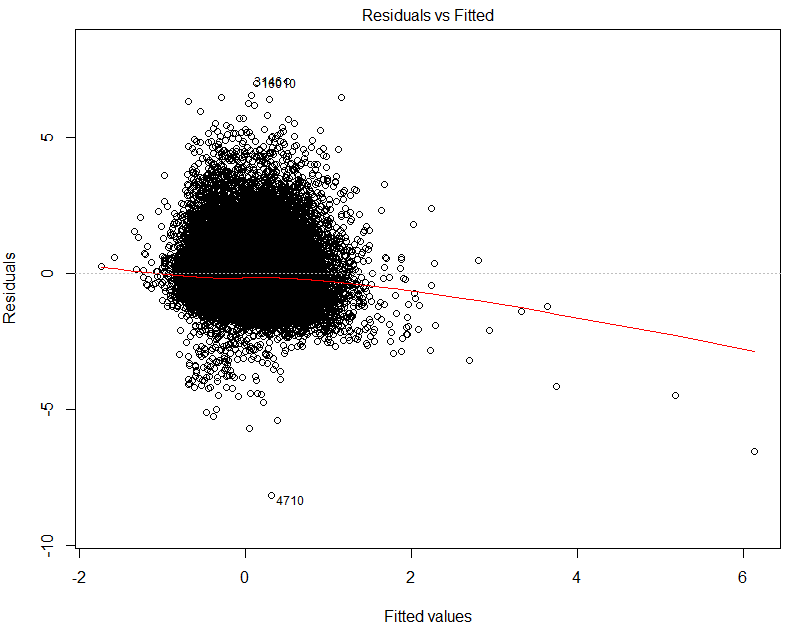
\includegraphics[width=0.7\linewidth]{linear_fvsr.png}
        \caption{Linear Regression Plot: Fitted vs Residuals}
        \label{fig:frp}
    \end{figure}  
    
    \begin{figure}[h]
        \centering
        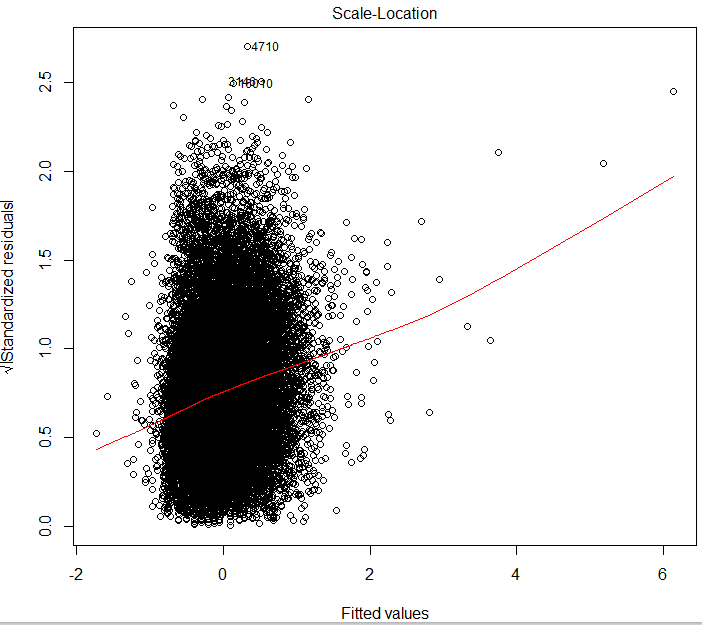
\includegraphics[width=0.7\linewidth]{linear_sl.png}
        \caption{Linear Regression Plot: Scale-location}
        \label{fig:sclo}
    \end{figure}
    
First, the residual vs. fitted plot in Figure \ref{fig:frp} and the Scale-location plot in Figure \ref{fig:sclo}. The latter plot is designed to check for nonconstant variance only. It uses the square root of standardized residuals by variance vs fitted values to show if residuals are spread equally along the ranges of predictors. If we can see a red horizontal line with equally randomly spread points in this plot, we can say that the assumptions is correct. From Figure \ref{fig:frp} we can see that most of points are in the left part, only few of them in the right part. Roughly speaking, the points seems symmetric when the fitted values are small, but perform somehow badly when fitted values are large. So we can think there is no non-linear relationships. In Figure \ref{fig:sclo}, we can see the red line is continually going up, which suggests that the assumptions of equal variance of the residuals may not be true. 

    \begin{figure}[h]
        \centering
        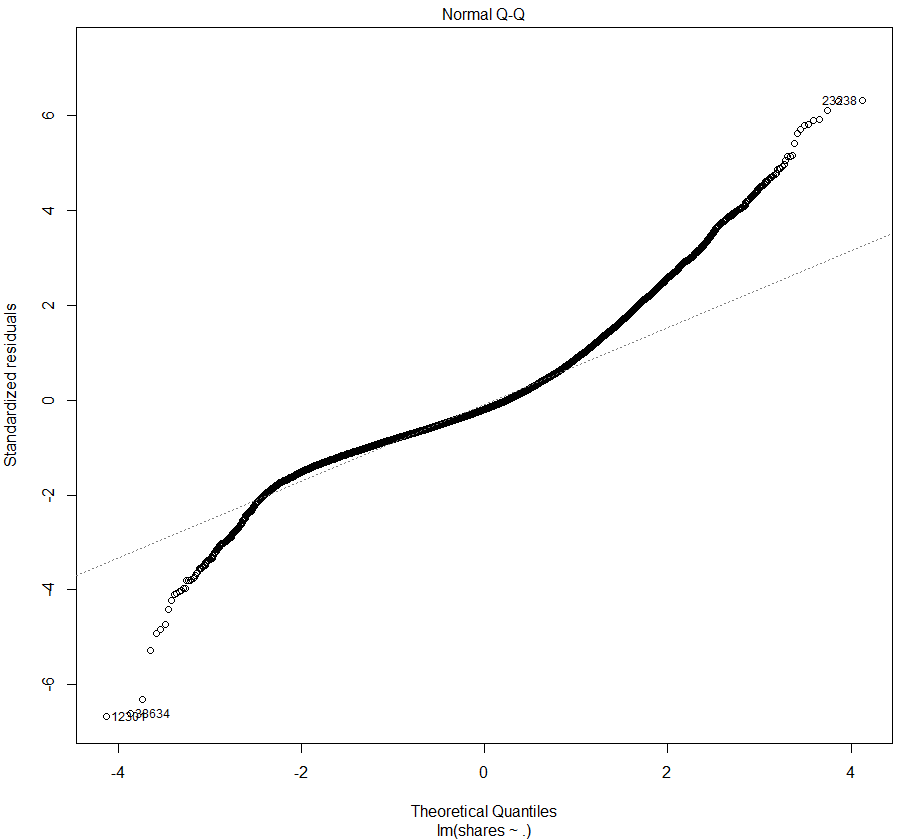
\includegraphics[width=0.7\linewidth]{linear_qq.png}
        \caption{Linear Regression Plot: QQ plot}
        \label{fig:qqp}
    \end{figure}    
    
    The tests and confidence intervals we use are base on the assumption of normal errors. We can check the residual normality using a Q-Q plot. This compares the residuals to some "ideal" observations from normal distribuion. So we plot all sorted residuals against $\Phi^{-1}(\frac{i}{n+1})$ for i = 1,2,...,n. See the Q-Q plot of Figure \ref{fig:qqp}, we can see a line, normal residuals should follow this line approximately. It shows that the residuals are not normally distributed so well. So we should have a concern about the residuals distribuion.\\
    
    We can use a quantity called the variance inflation factor (VIF) to get the collinearity for each variable. Let $R^2_j$ be the square of the multiple correlation coefficient that results when the predictor variable $X_j$ is regressed against all the other predictor variables. Then $$\text{VIF}(X_j) = \frac{1}{1 - R^2_j}, \quad j = 1, ... , p.$$ So if $X_j$ has a strong linear relationship with the other predictor variables, $R^2_j \to 1$ and $\text{VIF}(X_j) \to \infty$. Values of VIF greater than 10 is often taken as a signal that the data have collinearity problems.\cite{vif} So for all variables, I calculate the VIF for each of the variable, and some of their VIF value are larger than 10, which shows the collinearity is significant in these variables. And we maybe can think about remove them. \\ 
    
\subsection{Result}
\subsubsection{Regression}
Before doing any analysis on data, we use boxplot to look around all variables. And we find something observations need to be removed like the Figure \ref{fig:boxplot}. As the variable n{\_}non{\_}stop{\_}words is the rate of non-stop words in the content, it’s really wired that all the words in one articles are all stop words like the or a. So after removing some observations, we think the data should be good to analysis.

\begin{figure}[h]
    \centering
    \begin{subfigure}[h]{0.4\textwidth}
        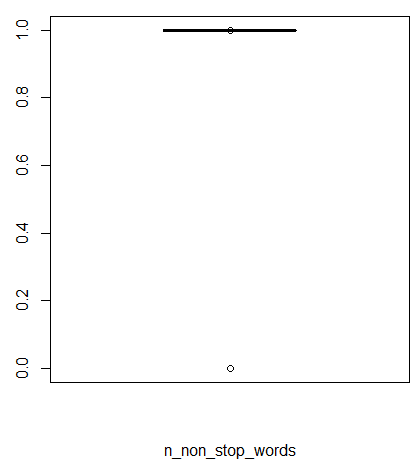
\includegraphics[width=\textwidth]{data-c4.png}
        \caption{Before}
    \end{subfigure}
    ~ %add desired spacing between images, e. g. ~, \quad, \qquad, \hfill etc. 
      %(or a blank line to force the subfigure onto a new line)
    \begin{subfigure}[h]{0.4\textwidth}
        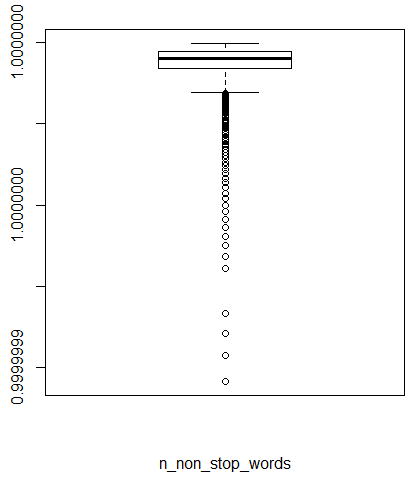
\includegraphics[width=\textwidth]{data-c5.png}
        \caption{After}
    \end{subfigure}
    \caption{Boxplot of the rate of non-stop words in the content}
    \label{fig:boxplot}
\end{figure}

To compare each method result, we decide to separate the whole dataset into training and testing part. We use 70\% of the data to train each model, and then use the rest one to test the error. For regression model, we compare the MSPE among linear regression, lasso and GAM. Before training the model, we look at the distribution of the number of shares, it seems like the log of number of shares follows normal distribution. So we normalize the log of number of shares and other variables by their mean and variance.\\

    \begin{figure}[h]
        \centering
        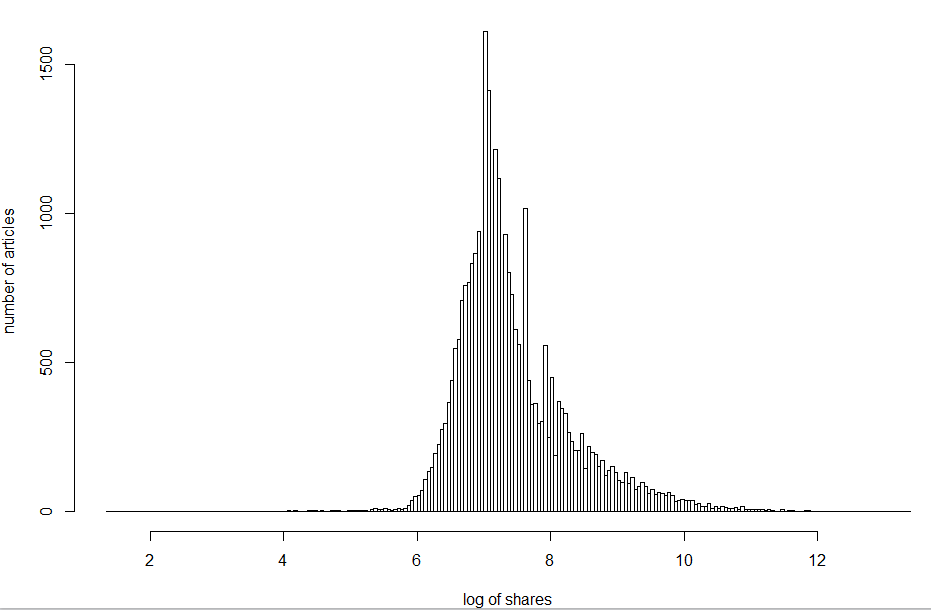
\includegraphics[width=0.85\linewidth]{logy.png}
        \caption{Histogram of log(shares) in training dataset}
        \label{fig:logy}
    \end{figure}

For the linear regression model, we use all variables including the variable timedelta which is describing the days between the article publication and the dataset acquisition. We get MSPE of 1.255954. \\

The lasso gives the MSPE of 1.25917. We use cross-validation method first to decide the lambda, after the cross-validation, we use the lambda that gives the minimum MSE to train the model, then get the MSPE. As we can see from Figure \ref{fig:lasso}, the left vertical dash line is the lambda that gives minimum MSE, and the right one is the largest value of lambda such that error is within one standard error of minimum. The number above Figure \ref{fig:lasso} is the number of features chosen by lasso. \\

    \begin{figure}[h]
        \centering
        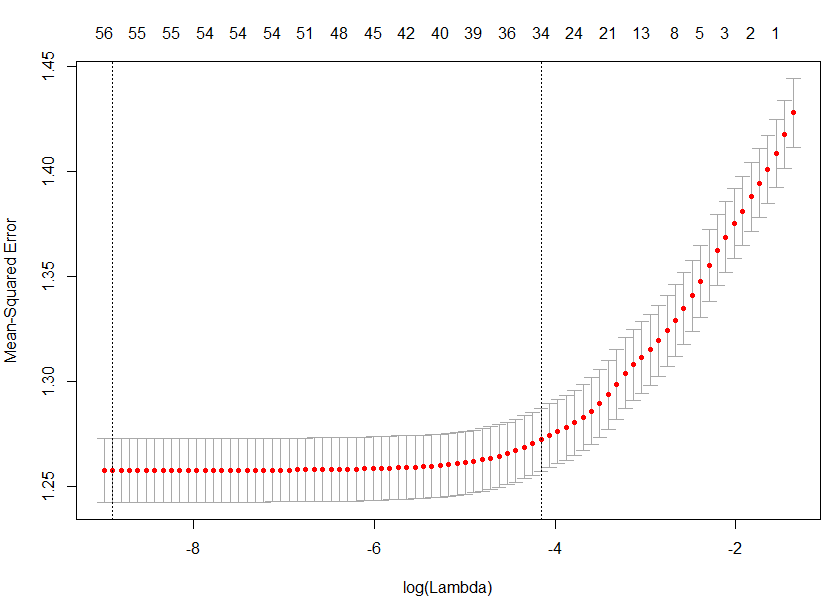
\includegraphics[width=0.7\linewidth]{lasso_plot.png}
        \caption{lasso}
        \label{fig:lasso}
    \end{figure}
    
For GAM, we try to apply smoothing splines to numeric variables. Firstly, we tried the smoothing splines with degree of freedom from 1 to 8. Using cross-validation method, we get the best model is when the degree of freedom is 6 (See from Figure \ref{fig:gam}). After choose the degree of freedom, we get the MSPE 1.211481. \\ 

    \begin{figure}[h]
        \centering
        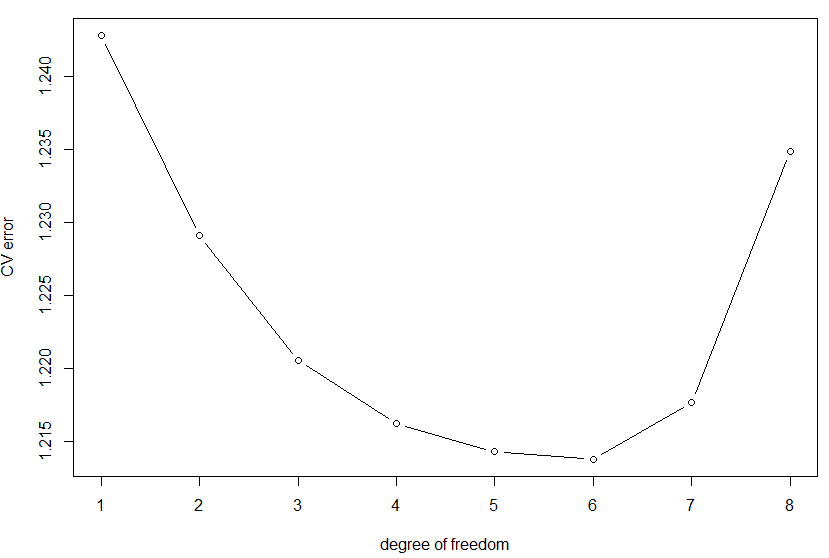
\includegraphics[width=0.9\linewidth]{gam_plot.png}
        \caption{GAM with smoothing spline with different degree of freedom}
        \label{fig:gam}
    \end{figure}

    \begin{table}[h]
        \centering
        \caption{MSPE for Regression}
        \begin{tabular}{ l | r }
            \hline\hline
            Regression model & Testing MSPE\\
            \hline
            linear regression & 1.255954 \\
            lasso & 1.25917 \\
            GAM & 1.211481 \\
            \hline\hline
        \end{tabular}
        \label{table:1}
    \end{table}

From the regression models, we can find that the MSPEs are not so different from each other. We can't tell which is the best by only looking at the testing MSPE. As we think that the exact share number is not a big deal when the number of share is extreme large or extreme small, we can split the response into three categorical level, and give a classification prediction.

\subsubsection{Classification}
From the Figure \ref{fig:logy}, we can see that the response of this dataset is normal distributed. So 
most of the articles have a very normal number of shares, only a few articles have very large or small number of shares. According to the training dataset, we decide to label the number of shares into three levels (unpopular, normal and popluar) shown in Table \ref{table:Popularity}. \\
    \begin{table}[h]
        \centering
        \caption{Popularity categories}
        \begin{tabular}{ l | r }
            \hline\hline
            The interval of log(shares) & Popularity\\
            \hline
            $\left[$0, 6.6746) & Unpopular \\
            $\left[$6.6746, 8.3894) & Normal \\
            $\left[$8.3894, $\infty$) & Popular \\
            \hline\hline
        \end{tabular}
        \label{table:Popularity}
    \end{table}

    \begin{figure}[h]
        \centering
        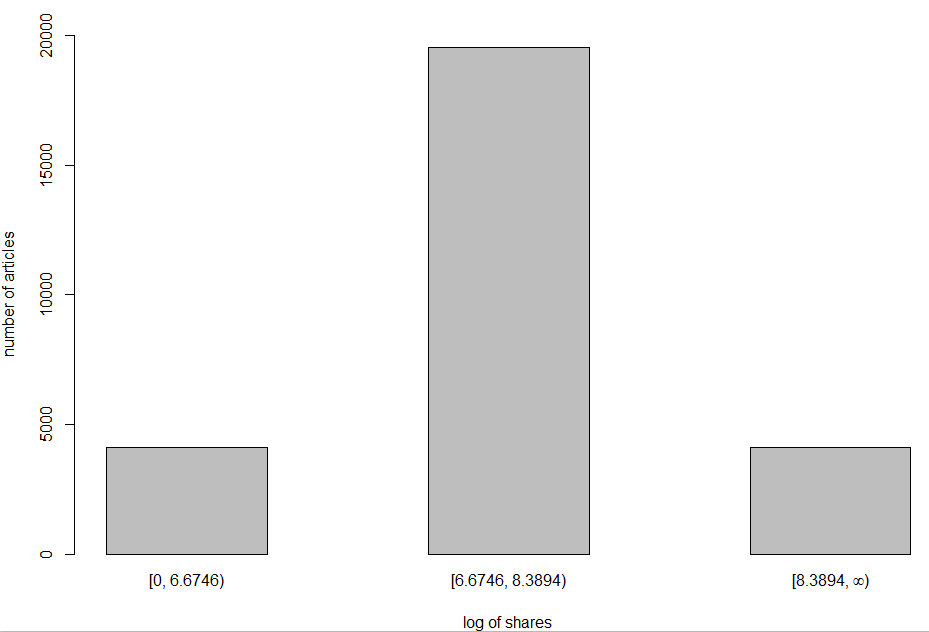
\includegraphics[width=0.8\linewidth]{poplularity.png}
        \caption{Popularity categories}
    \end{figure}

For the one vs one SVM model, we try two different kernel, linear or radial. For the linear kernel, we try C = 0.1, 1, 10, 100, 1000, and use the 10-fold cross-validation method in the training dataset to get the best value for parameter C is 0.1. And we also use the radical method and try C = 0.1, 1, 10, 100, 1000 together with $\gamma$ = 0.25, 0.5, 1, 2, 4. Then we still use the 10-fold cross-validation method to get the best C = 0.1 and $\gamma$ = 0.25. So we can find the testing accuracy is 0.7028 from radical .

    \begin{table}[h]
        \centering
        \caption{Confusion Matrix for SVM (radical kernel, C = 0.1, $\gamma$ = 0.25)}
        \begin{tabular}{ c | c | c | c | c }
            \hline\hline
            {} & \multicolumn{4}{c}{Reference} \\
            \hline
            Predition & Unpopular & Normal & Popular & Accuracy\\
            \hline
            Unpopular & 0 & 0 & 0 & NaN\\
            \hline
            Normal & 1754 & 8108 & 1675 & 0.7028\\
            \hline
            Popular & 0 & 0 & 0 & NaN\\
            \hline\hline
        \end{tabular}
        \label{table:knn}
    \end{table}

The random forest gives the accuracy 0.7021 with m = 5. We can try the number of variables from 1 to 56, and build 2000 trees. We use cross-validation method to figure out the number of variables that we should selected at random from the 56 variables. We can find that when m = 5 will give the best accuracy in the training dataset. 

    \begin{figure}[h]
        \centering
        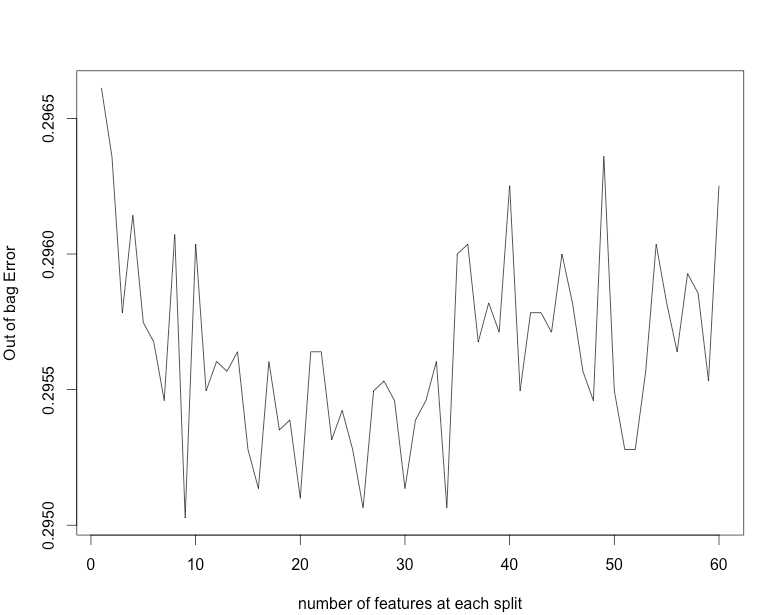
\includegraphics[width=0.8\linewidth]{randomforest_oob.png}
        \caption{Cross-validation error for random forest with different m}
    \end{figure}
    
    \begin{table}[h]
        \centering
        \caption{Confusion Matrix for random forest (m = 5)}
        \begin{tabular}{ c | c | c | c | c }
            \hline\hline
            {} & \multicolumn{4}{c}{Reference} \\
            \hline
            Predition & Unpopular & Normal & Popular & Accuracy\\
            \hline
            Unpopular & 21 & 19 & 0 & 0.525000\\
            \hline
            Normal & 1732 & 8062 & 1658 & 0.70398\\
            \hline
            Popular & 1 & 27 & 17 & 0.377778\\
            \hline\hline
        \end{tabular}
        \label{table:rf}
    \end{table}

The confusion matrix in Table \ref{table:rf} shows that we can predict Unpopular fairly well, and Normal and Popular can still be predicted correct for the majority.

For KNN, we try k from 1 to 100, which means we wish to find the best number of points in dataset to represent the point we want to predict. We use the cross-validation method to get the accuracy for every k value, and find out that best number of points is 17. We get the testing accuracy for KNN is 0.6965.

    \begin{figure}[h]
        \centering
        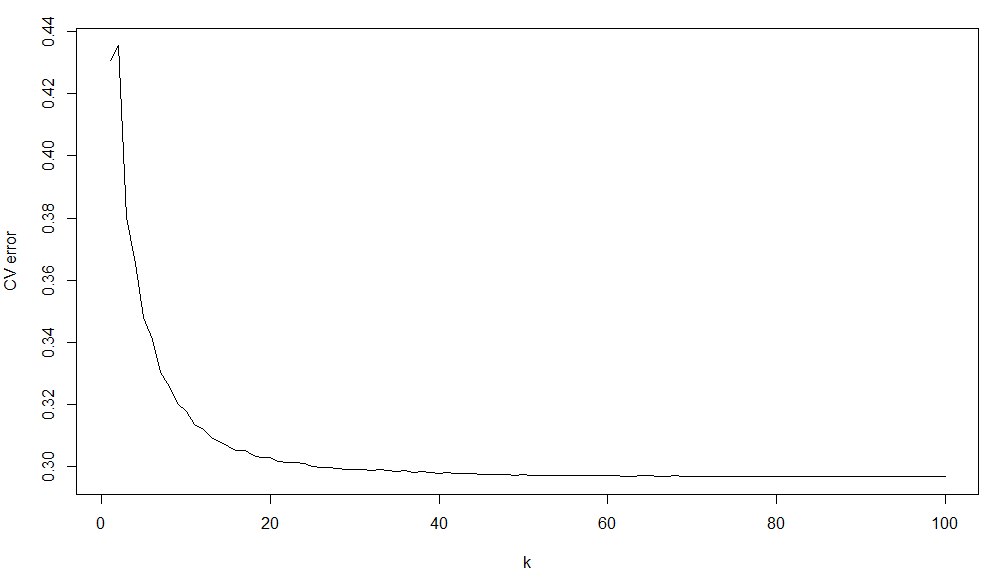
\includegraphics[width=0.7\linewidth]{knn_cv.png}
        \caption{Cross-validation error for KNN with differnent k}
    \end{figure}

    \begin{table}[h]
        \centering
        \caption{Confusion Matrix for KNN (k = 17)}
        \begin{tabular}{ c | c | c | c | c }
            \hline\hline
            {} & \multicolumn{4}{c}{Reference} \\
            \hline
            Predition & Unpopular & Normal & Popular & Accuracy\\
            \hline
            Unpopular & 94 & 155 & 21 & 0.348148\\
            \hline
            Normal & 1657 & 7925 & 1638 & 0.70633\\
            \hline
            Popular & 3 & 28 & 16 & 0.340426\\
            \hline\hline
        \end{tabular}
        \label{table:knn}
    \end{table}

The confusion matrix in Table \ref{table:knn} shows that this method is not as good as random forest in Unpopular and Popular part, but Normal can still be predicted correct for the majority.

    \begin{table}[h]
        \centering
        \caption{Accuracy for classification}
        \begin{tabular}{ l | r }
            \hline\hline
            Classification model & Accuracy\\
            \hline
            SVM & 0.7028 \\
            Random forest & 0.7021 \\
            KNN & 0.6965 \\
            \hline\hline
        \end{tabular}
        \label{table:1}
    \end{table}


\clearpage
\section{Conclusion}
In this thesis, we train several regression and classification models to predict the popularity of some online articles before them are published. We use number of shares to judge the popularity of the articles. The data we use is from Mashable news service, providing from UCI Machine Learning Repository.  \\
Over the regression models, the best result was achieved by Generalized Additive Model(GAM) with a testing mean squared error 1.225438 after the normalization for the log of number of shares. As we know, linear regression and lasso are not flexible compared with GAM, which means they are supposed to get a bigger MSE but less variance. As diagnostics we have done, it shows that the variables are more possible having a non-linear relationship with response. So I think the non-linear model such as GAM could be a good fit for the regression model. \\
As the classification models, the best result goes to random forest with the accuracy 0.4458085. Looking through the confusion matrix, we can find out that only random forest can give a prediction for those articles labeled by Unpopular or Popular.\\
Overall, the work for this thesis gives a new perspective about the reason for influencing the popularity of online articles from a statistics view instead of content or article style. \\
In the future work, we want to use the method that the orginal thesis gives to get more data from other online articles resources to train a better model, and also try to use more method to give a better prediction.

\clearpage
\section{Appendix}
\singlespacing
    \begin{table}[h]
        \centering
        \footnotesize
        \caption{List of variables}
        \begin{tabular}{ l | l }
            \hline\hline
            Variable names & Type(\#)\\
            \hline
            \multicolumn{2}{c}{Words}\\
            \hline
            Number of words in the title & numeric(1) \\
            Number of words in the content & numeric(1) \\
            Average length of the words in the content & numeric(1) \\
            Rate of unique words in the content & numeric(1) \\
            Rate of non-stop words in the content & numeric(1) \\
            Rate of unique non-stop words in the content & numeric(1) \\
            \hline
            \multicolumn{2}{c}{Links}\\
            \hline
            Number of links & numeric(1) \\
            Number of links to other articles published by Mashable & numeric(1) \\
            Shares of referenced article links in Mashable (min, avg, max) & numeric(3) \\
            \hline
            \multicolumn{2}{c}{Digital Media}\\
            \hline
            Number of images & numeric(1) \\
            Number of videos & numeric(1) \\
            \hline
            \multicolumn{2}{c}{Time}\\
            \hline
            Days between the article publication and the dataset acquisition & numeric(1) \\
            Day of the week (from Monday to Sunday) & binary(7) \\
            The article published on the weekend & binary(1) \\
            \hline
            \multicolumn{2}{c}{Keywords}\\
            \hline
            Number of keywords in the metadata & numeric(1) \\
            Data channel (Lifestyle, Entertainment, Business, Social Media, Tech or World) & binary(6) \\
            Worst keyword shares (min, avg, max) & numeric(3) \\
            Best keyword shares (min, avg, max) & numeric(3) \\
            Average keyword shares (min, avg, max) & numeric(3) \\
            \hline
            \multicolumn{2}{c}{Natural Language Processing}\\
            \hline
            Closeness to top LDA topics from 1 to 5 & numeric(5) \\
            Text subjectivity & numeric(1) \\
            Text sentiment polarity & numeric(1) \\
            Rate of positive words in the content & numeric(1) \\
            Rate of negative words in the content & numeric(1) \\
            Rate of positive words among non-neutral tokens & numeric(1) \\
            Rate of negative words among non-neutral tokens & numeric(1) \\
            Polarity of positive words (min, avg, max) & numeric(3) \\
            Polarity of negative words (min, avg, max) & numeric(3) \\
            Title subjectivity & numeric(1) \\
            Title polarity & numeric(1) \\
            Absolute subjectivity level & numeric(1) \\
            Absolute polarity level & numeric(1) \\
            \hline\hline
        \end{tabular}
        \label{table:1}
    \end{table}
\clearpage

\doublespacing

\addcontentsline{toc}{section}{References}
\bibliographystyle{plain}
\bibliography{biblio}
\end{document}